%% proposal-dataV2.tex
%% Generated from proposal-dataV2.docx
%% Compile with:  pdflatex proposal-dataV2  (run twice for cross references)
%% Images are stored in ./proposal-dataV2-figures/ and referenced via \graphicspath.

\documentclass[11pt,a4paper]{article}

% ---------- Encoding & fonts ----------
\usepackage[T1]{fontenc}
\usepackage[utf8]{inputenc}
\usepackage{lmodern}
\usepackage{microtype}

% ---------- Layout ----------
\usepackage[margin=1in]{geometry}
\usepackage{setspace}
\onehalfspacing

% ---------- Graphics & tables ----------
\usepackage{graphicx}
\graphicspath{{proposal-dataV2-figures/}}
\usepackage{booktabs}
\usepackage{longtable}
\usepackage{array}
\usepackage{multirow}
\usepackage{caption}
\captionsetup{font=small,labelfont=bf}

% ---------- Lists / links ----------
\usepackage{enumitem}
\usepackage[hidelinks]{hyperref}

% ---------- Convenience ----------
\newcolumntype{L}[1]{>{\raggedright\arraybackslash}p{#1}}
\setlength{\parindent}{0pt}
\setlength{\parskip}{0.6em}

\title{%
  \textbf{\large AI for Materials Discovery: A Data-Centric Perspective}%
}
\author{}
\date{}

\begin{document}
\maketitle
\thispagestyle{empty}

% =====================================================================
% In-brief / Blurb
% =====================================================================
\begin{abstract}
\small
Artificial Intelligence holds immense potential to accelerate materials
discovery, yet translating this potential into scientific advances depends
on the data that underpin model development and experimental validation.
While existing reviews largely emphasize models and methods, a systematic
assessment of how existing data resources support the progression from
prediction to experimentally validated materials discovery remains needed.
This review examines progress in AI-driven materials discovery through the
lens of data and establishes principles for building data foundations that
bridge the gap between predictive capability and experimentally validated
discovery.
\end{abstract}

\vspace{0.5em}
\noindent\textbf{Alternative titles under consideration:}
\begin{enumerate}[leftmargin=1.4em,itemsep=1pt,topsep=2pt]
  \item AI for Materials Discovery: A Data-Centric Perspective
  \item AI for Materials Discovery: A Data-Centered Review of Datasets and Benchmarks
  \item AI for Materials Discovery: Datasets, Benchmarks, and Evaluation Gaps
\end{enumerate}

% =====================================================================
% Abstract
% =====================================================================
\section*{Abstract}
Data form the scientific foundation of AI-driven materials discovery,
shaping what models can learn, which candidates they can propose, and how
computational predictions can inform experimental validation. From an AI
for Science perspective, this review examines the data foundations of
materials discovery through a two-dimensional taxonomy organized by
discovery tasks and data sources. Covering property prediction, generative
and inverse design, sequential optimization, closed-loop experimentation,
and scientific reasoning, we analyze how data generation, representation,
quality, coverage, and connectivity enable or constrain discovery. We map
existing data resources according to their support for increasingly complex
discovery tasks and their relevance to real-world materials research. This
analysis reveals persistent gaps in underexplored materials spaces,
synthesis and processing information, unsuccessful experiments,
uncertainty reporting, and records of iterative discovery processes. We
further examine how fragmented data practices and discrepancies between
computational and experimental evidence limit the translation of AI outputs
into validated materials. Finally, we propose principles for collecting,
curating, connecting, and maintaining discovery-relevant data, emphasizing
scientific context, provenance, interoperability, and continuous feedback
from experiments. These principles aim to strengthen the data foundations
needed to move materials AI from learning established relationships toward
guiding the discovery and validation of new materials.

% =====================================================================
% Brief description of the main article sections
% =====================================================================
\section*{Brief description of the main article sections}
The main article sections of this paper are as below.

% =====================================================================
\section{Introduction}
% =====================================================================
This section positions data as a scientific foundation of AI-driven
materials discovery. It explains how choices about what to measure,
compute, report, and preserve shape the knowledge available to AI and the
discovery activities it can support. It motivates a data-centric review
that connects existing data resources with the scientific requirements of
materials discovery, extending beyond data availability to consider
quality, context, connectivity, and practical utility.

\begin{figure}[htbp]
  \centering
  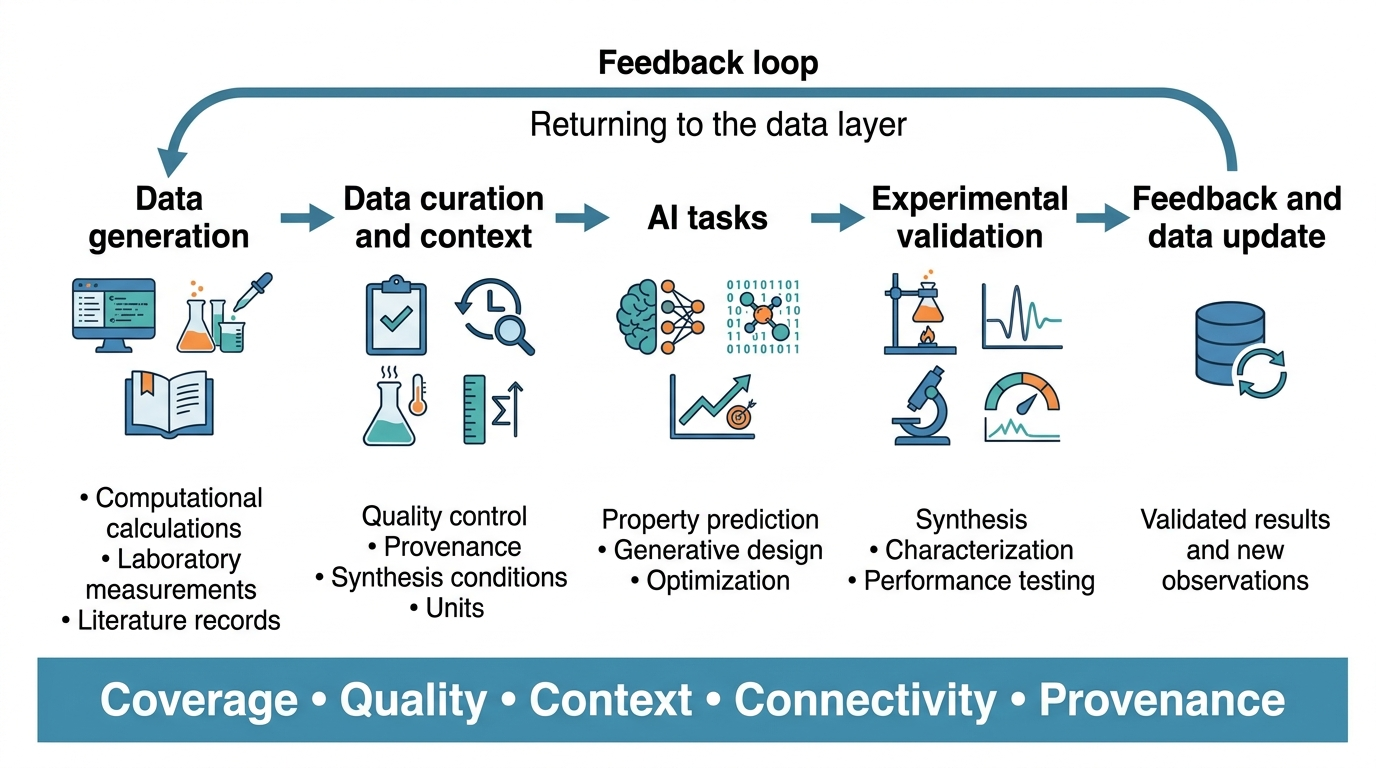
\includegraphics[width=0.95\textwidth]{fig1_introduction_framework.jpeg}
  \caption{Overview of the data-centric framing of AI for materials
  discovery: how materials datasets are transformed into AI tasks and
  benchmarks, and whether these resources support meaningful
  materials-discovery progressions.}
  \label{fig:introduction-framework}
\end{figure}

As shown in Figure~\ref{fig:introduction-framework}, this paper is a review
of how materials datasets are transformed into AI tasks and benchmarks, and
whether these resources support meaningful materials discovery.

Data are not merely inputs to AI for materials discovery; they define the
evidence from which models learn, the materials and properties they can
represent, and the extent to which predictions can guide experimental
validation. The coverage, quality, provenance, and connectivity of
materials data therefore shape not only model performance, but also the
kinds of discovery questions AI can address.

\paragraph{Data as the Foundation of AI for Materials Discovery.}
\paragraph{From Materials Datasets to Discovery Benchmarks.}

% =====================================================================
\section{A Taxonomy of Materials Discovery Datasets and Benchmarks}
% =====================================================================
This section introduces a taxonomy organized along two complementary
dimensions---materials discovery tasks and data sources---and uses it to
structure a comprehensive review of existing data sources.

\begin{figure}[htbp]
  \centering
  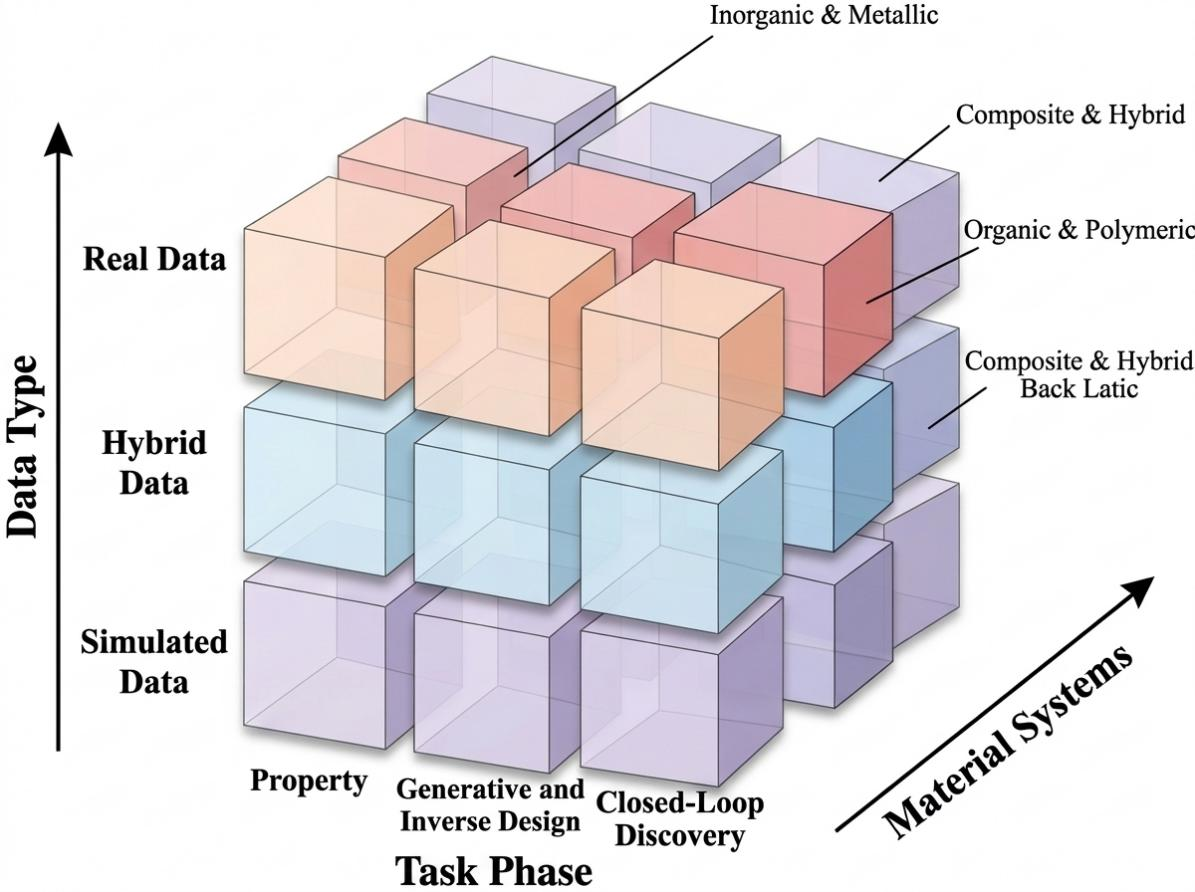
\includegraphics[width=0.95\textwidth]{fig2_taxonomy.jpeg}
  \caption{Taxonomy diagram of materials-discovery datasets and benchmarks.
  The horizontal axis represents the complexity of materials discovery
  tasks, ranging from Property Prediction to Generative and Inverse Design,
  and finally to Sequential Optimization and Closed-Loop Discovery. The
  vertical axis indicates the source of the data, categorised into
  simulated data, mixed data, and real-world data. Within each cell we
  summarise the relevant literature for different material systems based on
  our analysis, highlighting the key characteristics of the data.}
  \label{fig:taxonomy}
\end{figure}

Here, we present a taxonomy diagram (Figure~\ref{fig:taxonomy}) to give
readers a more intuitive overview of the structure of this review. Within
each category, we summarise the relevant literature in different material
systems based on our analysis, highlighting the key characteristics of the
data and helping readers better understand the corresponding research
landscape. The material systems covered are:

\begin{itemize}[leftmargin=1.4em,itemsep=2pt,topsep=2pt]
  \item \textbf{Inorganic Solid Materials}
  \item \textbf{Metallic Materials}
  \item \textbf{Organic and Polymeric Materials}
  \item \textbf{Other Material Systems}
\end{itemize}

% =====================================================================
\section{The Current Data Landscape}
% =====================================================================
This section maps the current data landscape along two dimensions: support
for discovery tasks of increasing complexity, and relevance to real-world
materials discovery. An LLM-assisted and human-validated annotation
protocol supports systematic comparison using explicit criteria and
traceable evidence, while accounting for incomplete documentation and
uncertainty.

We will construct a scoring \textsc{skill} to evaluate the collected
datasets. After evaluation by at least three large language models (LLMs),
we will invite at least two domain experts to further assess the datasets
and conduct a second-round verification of any datasets that receive
inconsistent scores. All evaluation reports will be made publicly available
alongside this review. The final score for each dataset will be calculated
as the average of the assigned scores.

\begin{figure}[htbp]
  \centering
  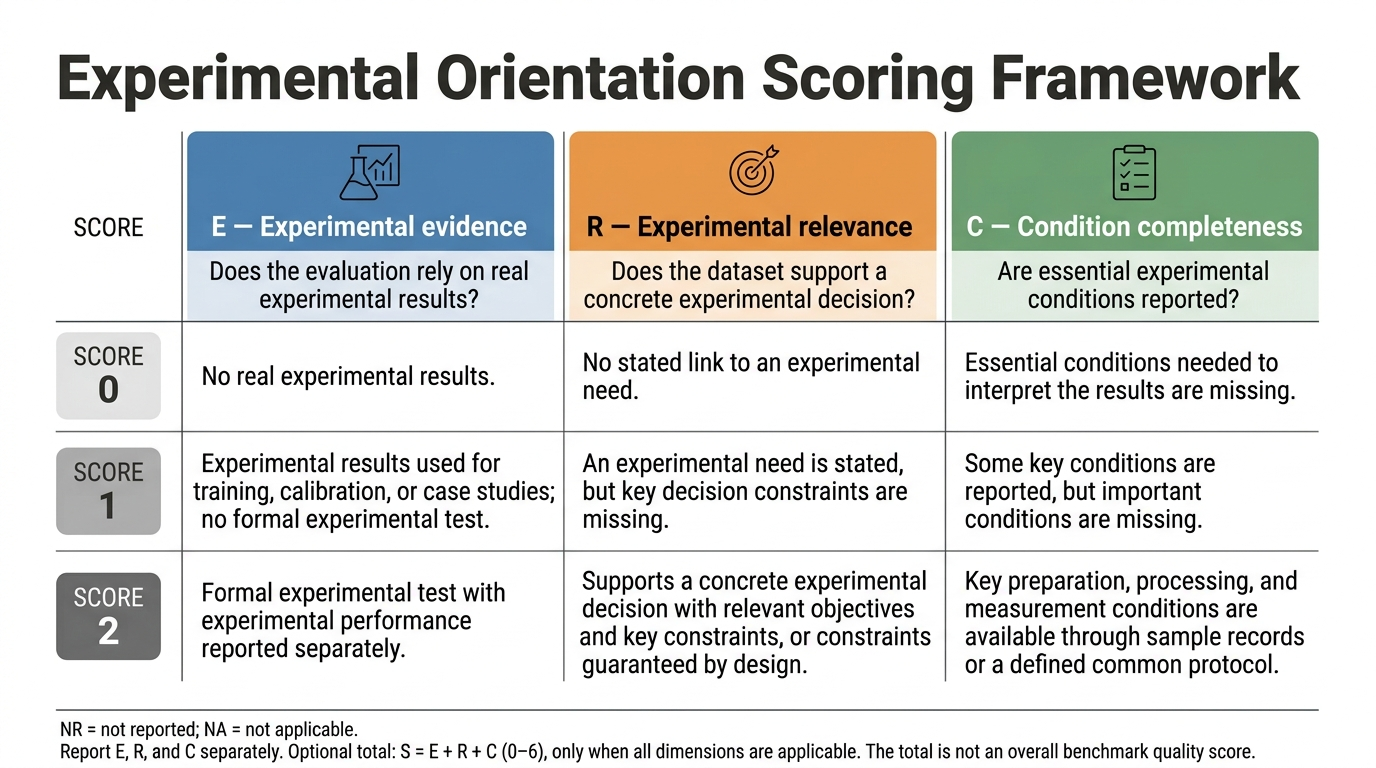
\includegraphics[width=0.95\textwidth]{fig3_data_landscape.jpeg}
  \caption{Current landscape of AI-oriented materials-discovery datasets,
  positioned by task complexity (horizontal) and data source / real-world
  relevance (vertical).}
  \label{fig:data-landscape}
\end{figure}

\subsection{The Data Evaluation Space}
This section represents existing datasets in a continuous evaluation space
defined by task-intelligence requirements (\emph{x}~axis) and real-world
discovery effectiveness (\emph{y}~axis) to reveal their overall
distribution, concentration, and unexplored regions.

\subsection{Coverage across Machine Learning Tasks}
This section (\emph{x}~axis) analyses how different machine-learning
paradigms are represented across current datasets, including supervised
learning, generative modelling, active learning, Bayesian optimisation,
reinforcement learning, and so on.

\subsection{Coverage across Materials Discovery Contexts}
This section (\emph{y}~axis) compares dataset coverage across material
domains, target properties, simulation and experimental settings, and
synthesis or validation contexts to identify systematic biases and gaps.

\begin{figure}[htbp]
  \centering
  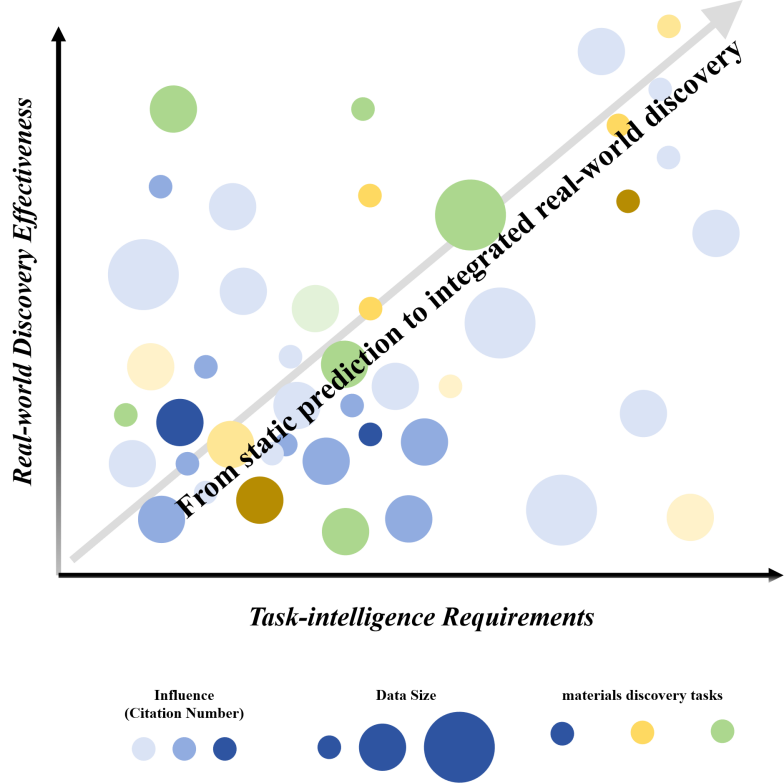
\includegraphics[width=0.9\textwidth]{fig4_score_heatmap_a.png}
  \caption{Evaluation scores of all datasets. Colour intensity encodes the
  influence of each dataset (measured by citation count); marker size
  encodes dataset scale; different colours correspond to different task
  types in the materials domain.}
  \label{fig:scores-a}
\end{figure}

\begin{figure}[htbp]
  \centering
  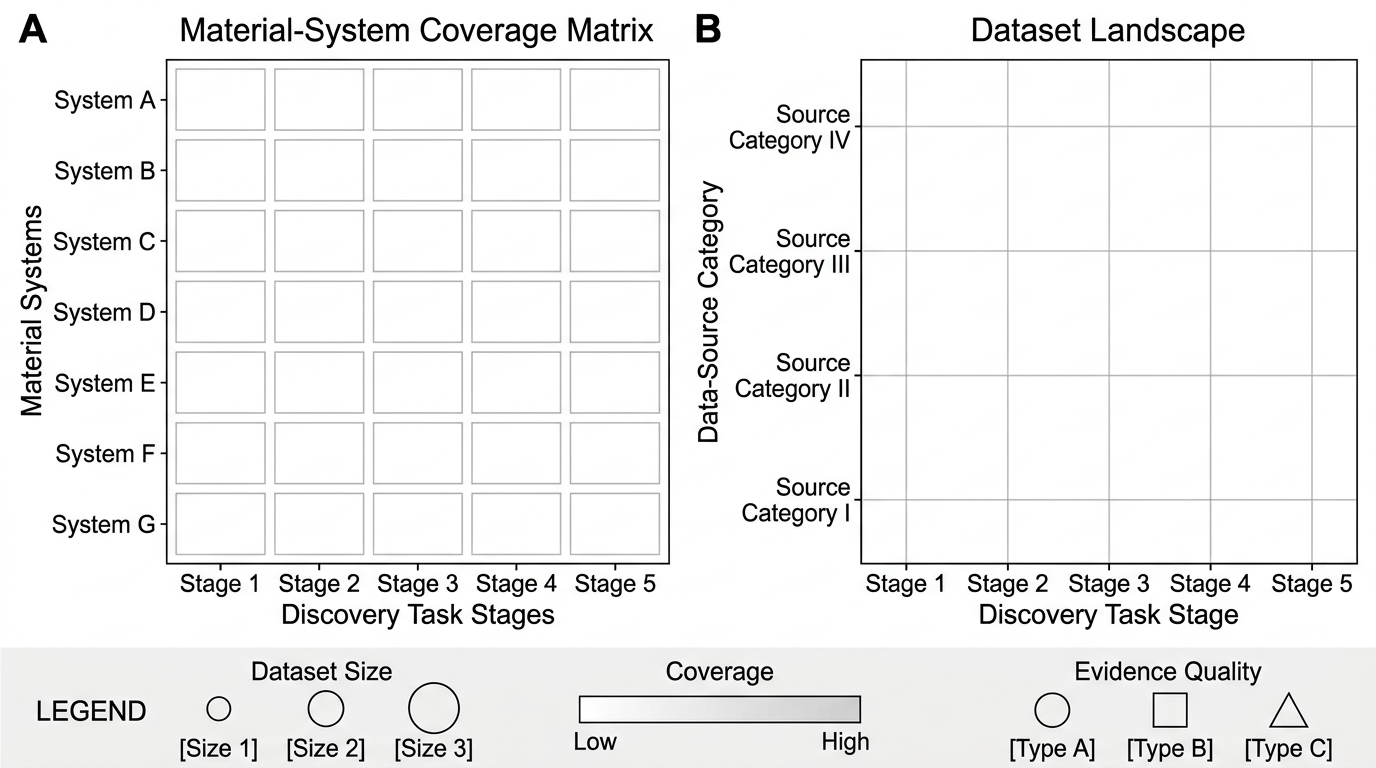
\includegraphics[width=0.9\textwidth]{fig5_score_visualization.jpeg}
  \caption{Companion view of the dataset-score distribution, providing an
  intuitive overview of the landscape of AI-enabled materials research and
  motivating the analyses in Sections 3--4.}
  \label{fig:scores-b}
\end{figure}

Here, we visualise the evaluation scores of all datasets
(Figures~\ref{fig:scores-a} and~\ref{fig:scores-b}). The colour intensity
represents the influence of each dataset, measured according to its
citation count; the size of each marker indicates the scale of the dataset;
and different colours correspond to different task types in the materials
domain. This visualisation provides an intuitive overview of the
distribution of datasets in AI-enabled materials research, offers a useful
reference for our dataset-centric review of AI capabilities, and motivates
the following questions and corresponding analyses.

% =====================================================================
\section{Discussion}
% =====================================================================
Building on the landscape analysis, this section examines whether current
data practices provide the evidence needed to make and validate
consequential materials-discovery decisions. It considers how data gaps,
loss of scientific context, and weak connections among records affect the
progression from identifying statistical relationships to proposing,
synthesising, and validating new materials.

\subsection{What Do Current Benchmarks Actually Measure?}
This section asks whether current benchmarks measure genuine
materials-discovery capabilities or merely performance on simplified,
static, and potentially biased prediction tasks.

\subsection{Do Available Data Support Real-World Discovery?}
This section examines how available data inform candidate selection,
synthesis planning, characterisation, and validation. It analyses barriers
arising from computational--experimental discrepancies, differences between
laboratory conditions, incomplete preparation details, and limited coverage
of unfamiliar materials. Drawing on documented discovery workflows, it
assesses where data have supported experimentally validated outcomes and
where additional evidence is needed to establish practical utility.

% =====================================================================
\section{Building Data Foundations for Materials Discovery}
% =====================================================================
This section proposes principles for collecting, curating, connecting, and
maintaining data around the requirements of materials discovery.

% =====================================================================
\section{Conclusion}
% =====================================================================
This section summarises the main findings, discusses the limitations of
current materials-discovery datasets, and outlines directions for
developing more intelligent, realistic, reproducible, and
discovery-relevant evaluation systems.

% =====================================================================
\appendix
\section*{Appendix: Dataset Metadata Schema}
% =====================================================================
We will provide descriptive metadata for each dataset, with the specific
fields listed in Table~\ref{tab:metadata-fields}. We will also
open-source the skills used for scoring.

\begin{longtable}{@{}L{4.2cm}L{9.6cm}@{}}
\caption{Descriptive metadata fields collected for every dataset reviewed
in this article.}\label{tab:metadata-fields} \\
\toprule
\textbf{Field} & \textbf{Description} \\
\midrule
\endfirsthead
\toprule
\textbf{Field} & \textbf{Description} \\
\midrule
\endhead
\bottomrule
\endfoot
Number                       & / \\
DOI                          & / \\
Paper Title                  & / \\
Task Code                    & Property Prediction, Generative Inverse Design, or Sequential Optimization and Closed-Loop Discovery \\
Data Type                    & Simulated data, mixed data, or real-world data \\
Real-world discovery effectiveness & Score vector \\
Task-intelligence requirements     & Score vector \\
Material System              & The material classes, chemical systems, or material domains represented in the dataset. \\
Input / Output               & A description of the input data provided to the model and the corresponding output or prediction target. \\
Modality Type                & The data modality or combination of modalities included in the dataset, such as text, numerical data, structures, images, spectra, or experimental records. \\
Data Source and Snapshot     & The origin of the dataset together with the version or snapshot date used in this review, so that results remain reproducible. \\
Dataset Size                 & The scale of the dataset, measured by the number of samples, records, or other relevant data units. \\
License                      & The legal terms and usage permissions governing access to, modification of, and redistribution of the dataset. \\
Citation                     & The number of citations received by the associated paper, used as an indicator of the dataset's academic influence. \\
Advantages                   & The main strengths and distinctive features of the dataset, such as its scale, quality, diversity, or practical relevance. \\
Notes                        & Additional information, clarifications, limitations, or special considerations relevant to the dataset. \\
\end{longtable}

% =====================================================================
\section*{Key References}
% =====================================================================
\begin{enumerate}[leftmargin=1.6em,itemsep=4pt,topsep=2pt]
  \item Dutra, A.~C.~C., Goldmann, B.~A., Islam, M.~S. et~al.
        Understanding solid-state battery electrolytes using atomistic
        modelling and machine learning.
        \emph{Nat.\ Rev.\ Mater.} \textbf{10}, 566--583 (2025).
  \item Xia, X., Leng, T., Garc\'{\i}a, A.~J. et~al.
        Machine learning for biomaterials design.
        \emph{Nat.\ Rev.\ Bioeng.} \textbf{4}, 881--899 (2026).
  \item Schumann, J., N\"asstr\"om, H., G\"otte, M. et~al.
        Enabling open and FAIR catalysis data with standardized data
        structures.
        \emph{Nat.\ Catal.} \textbf{9}, 225--229 (2026).
  \item Tran, H., Gurnani, R., Kim, C. et~al.
        Design of functional and sustainable polymers assisted by
        artificial intelligence.
        \emph{Nat.\ Rev.\ Mater.} \textbf{9}, 866--886 (2024).
\end{enumerate}

% =====================================================================
\section*{Authors}
% =====================================================================
\begin{table}[htbp]
  \centering
  \caption{Author names and their affiliations.}
  \begin{tabular}{@{}L{4.2cm}L{8.4cm}@{}}
    \toprule
    \textbf{Name} & \textbf{Institute} \\
    \midrule
    Chenglin Liu, Jian Xu   & Institute of Automation, Chinese Academy of Sciences (CASIA); Beijing Haidian Zhongguancun College \\
    Yanan Chen              & Tianjin University \\
    Bin Wang, Yang Gao      & National Center for Nanoscience and Technology (NCNST); Tibet University \\
    Jianjun Liu, Nian Ran   & Shanghai Institute of Ceramics, CAS \\
    Guixuan Wu              & Institute of Coal Chemistry, CAS \\
    \bottomrule
  \end{tabular}
\end{table}

\end{document}
